%%%%%%%%%%%%%%%%%%%%%%%%%%%%%%%%%%%%%%%%%
% Structured General Purpose Assignment
% LaTeX Template
%
% This template has been downloaded from:
% http://www.latextemplates.com
%
% Original author:
% Ted Pavlic (http://www.tedpavlic.com)
%
% Note:
% The \lipsum[#] commands throughout this template generate dummy text
% to fill the template out. These commands should all be removed when 
% writing assignment content.
%
%%%%%%%%%%%%%%%%%%%%%%%%%%%%%%%%%%%%%%%%%

%----------------------------------------------------------------------------------------
%	PACKAGES AND OTHER DOCUMENT CONFIGURATIONS
%----------------------------------------------------------------------------------------

\documentclass{article}

\usepackage{fancyhdr} % Required for custom headers
\usepackage{lastpage} % Required to determine the last page for the footer
\usepackage{extramarks} % Required for headers and footers
\usepackage{graphicx} % Required to insert images
\usepackage{lipsum} % Used for inserting dummy 'Lorem ipsum' text into the template
\usepackage{amsmath,amsfonts,amsthm} % Math packages

% Margins
\topmargin=-0.45in
\evensidemargin=0in
\oddsidemargin=0in
\textwidth=6.5in
\textheight=9.0in
\headsep=0.25in 

\linespread{1.1} % Line spacing

% Set up the header and footer
\pagestyle{fancy}
\lhead{\hmwkAuthorName} % Top left header
\chead{\hmwkClass\ (\hmwkClassInstructor\ \hmwkClassTime): \hmwkTitle} % Top center header
\rhead{\firstxmark} % Top right header
\lfoot{\lastxmark} % Bottom left footer
\cfoot{} % Bottom center footer
\rfoot{Page\ \thepage\ of\ \pageref{LastPage}} % Bottom right footer
\renewcommand\headrulewidth{0.4pt} % Size of the header rule
\renewcommand\footrulewidth{0.4pt} % Size of the footer rule

\setlength\parindent{0pt} % Removes all indentation from paragraphs

%----------------------------------------------------------------------------------------
%	DOCUMENT STRUCTURE COMMANDS
%	Skip this unless you know what you're doing
%----------------------------------------------------------------------------------------

% Header and footer for when a page split occurs within a problem environment
\newcommand{\enterProblemHeader}[1]{
\nobreak\extramarks{#1}{#1 continued on next page\ldots}\nobreak
\nobreak\extramarks{#1 (continued)}{#1 continued on next page\ldots}\nobreak
}

% Header and footer for when a page split occurs between problem environments
\newcommand{\exitProblemHeader}[1]{
\nobreak\extramarks{#1 (continued)}{#1 continued on next page\ldots}\nobreak
\nobreak\extramarks{#1}{}\nobreak
}

\setcounter{secnumdepth}{0} % Removes default section numbers
\newcounter{homeworkProblemCounter} % Creates a counter to keep track of the number of problems

\newcommand{\homeworkProblemName}{}
\newenvironment{homeworkProblem}[1][Problem \arabic{homeworkProblemCounter}]{ % Makes a new environment called homeworkProblem which takes 1 argument (custom name) but the default is "Problem #"
\stepcounter{homeworkProblemCounter} % Increase counter for number of problems
\renewcommand{\homeworkProblemName}{#1} % Assign \homeworkProblemName the name of the problem
\section{\homeworkProblemName} % Make a section in the document with the custom problem count
\enterProblemHeader{\homeworkProblemName} % Header and footer within the environment
}{
\exitProblemHeader{\homeworkProblemName} % Header and footer after the environment
}

\newcommand{\problemAnswer}[1]{ % Defines the problem answer command with the content as the only argument
\noindent\framebox[\columnwidth][c]{\begin{minipage}{0.98\columnwidth}#1\end{minipage}} % Makes the box around the problem answer and puts the content inside
}

\newcommand{\homeworkSectionName}{}
\newenvironment{homeworkSection}[1]{ % New environment for sections within homework problems, takes 1 argument - the name of the section
\renewcommand{\homeworkSectionName}{#1} % Assign \homeworkSectionName to the name of the section from the environment argument
\subsection{\homeworkSectionName} % Make a subsection with the custom name of the subsection
\enterProblemHeader{\homeworkProblemName\ [\homeworkSectionName]} % Header and footer within the environment
}{
\enterProblemHeader{\homeworkProblemName} % Header and footer after the environment
}
   
%----------------------------------------------------------------------------------------
%	NAME AND CLASS SECTION
%----------------------------------------------------------------------------------------

\newcommand{\hmwkTitle}{Homework\ \#5} % Assignment title
\newcommand{\hmwkDueDate}{Monday,\ November\ 11,\ 2013} % Due date
\newcommand{\hmwkClass}{CS4642} % Course/class
\newcommand{\hmwkClassTime}{3:00pm} % Class/lecture time
\newcommand{\hmwkClassInstructor}{Hongyuan Zha} % Teacher/lecturer
\newcommand{\hmwkAuthorName}{Nathan Korzekwa} % Your name

%----------------------------------------------------------------------------------------
%	TITLE PAGE
%----------------------------------------------------------------------------------------

\title{
\vspace{2in}
\textmd{\textbf{\hmwkClass:\ \hmwkTitle}}\\
\normalsize\vspace{0.1in}\small{Due\ on\ \hmwkDueDate}\\
\vspace{0.1in}\large{\textit{\hmwkClassInstructor\ \hmwkClassTime}}
\vspace{3in}
}

\author{\textbf{\hmwkAuthorName}}
\date{} % Insert date here if you want it to appear below your name

%----------------------------------------------------------------------------------------

\begin{document}

\maketitle

%----------------------------------------------------------------------------------------
%	TABLE OF CONTENTS
%----------------------------------------------------------------------------------------

%\setcounter{tocdepth}{1} % Uncomment this line if you don't want subsections listed in the ToC

\newpage
\tableofcontents
\newpage

%----------------------------------------------------------------------------------------
%	PROBLEM 1
%----------------------------------------------------------------------------------------

% To have just one problem per page, simply put a \clearpage after each problem
``Your trivial words of sorrow, of love and guilt mean nothing to me, young lady. My wife understands. She is the one that I chose to live by my side. There are no more words that need to pass between us now. That's what it means to be the wife of the Fuhrer." -- Fuhrer-President King Bradley
\begin{homeworkProblem}[Problem 1]

\begin{homeworkSection}{(a)} % Section within problem
	$$g_1^\prime(x) = 1 - 2x$$\\
	$$x^\star = \sqrt{3}$$
	A fixed-point function is locally convergent if and only if its magnitude of derivative at $x^\star$ is less than one.\\
	So, \\
	$$g_1^\prime(x^\star) = 1 - 2\sqrt{3}$$ \\
	and since we know $2 > \sqrt{3} > 1$,
	$$|g_1^\prime(x^\star)| > 1$$
	Therefore, this function is NOT locally convergent for $y = 3$.
	
\end{homeworkSection}

\begin{homeworkSection}{(b)} % Section within problem
	\begin{align*}
		g_2^\prime(x) &= 1 - \frac{2x}{y} \\
					  &= 1 - \frac{2x}{3} \\
	\end{align*}
	\begin{align*}
		x^\star &= \sqrt{3} \\
		x^\star &\ \epsilon \ (1, 2) \\
	\end{align*}
	therefore, because $g_2^\prime$ is a linear function of $x$, 
	\begin{align*}
		g_2^\prime(x^\star) &\ \epsilon \ (\frac{1}{3}, -\frac{1}{3}) \\
	\end{align*}
	
	From this, we must conclude that $|g_2^\prime(x^\star)| < 1$, meaning that this function has an interval of local convergence for $y = 3$.
\end{homeworkSection}

\begin{homeworkSection}{(c)} % Section within problem
	Since the function we are trying to find the root of is $f(x) = x^2 - 3 = 0$, and since Newton's method defines a fixed-point function as $g(x) = x - \frac{f(x)}{f^\prime(x)}$, the function for this problem is:
	$$
		g_n(x) = x - \frac{x^2 - y}{2x}
	$$
\end{homeworkSection}


\end{homeworkProblem}
\clearpage
%----------------------------------------------------------------------------------------
%	PROBLEM 2
%----------------------------------------------------------------------------------------

\begin{homeworkProblem}[Problem 2] % Custom section title
%--------------------------------------------
\begin{homeworkSection}{(a)} % Section within problem
	To determine what $d$ needs to be for this function to be locally convergent in terms of fixed-point iteration, we can apply the same logic as used in the previous section. Since we're assuming a global $d$, here, the following property must hold:
	\begin{align*}
		g^\prime(x^\star)= 1 - \frac{f^\prime(x^\star)}{d}\\
		|g^\prime(x^\star)| < 1
	\end{align*}
	From this, we can do some manipulation to get a range of valid values for $d$.
	
	\begin{align*}
		|1 - \frac{f^\prime(x^\star)}{d}| < 1 \\
		0 < \frac{f^\prime(x^\star)}{d} < 2 \\
		0 < \frac{1}{d} < \frac{2}{f^\prime(x^\star)} \\
		\infty > d > \frac{f^\prime(x^\star)}{2} \\
	\end{align*}
	
	So, this scheme will be locally convergent when $d > \frac{f^\prime(x^\star)}{2}$.
\end{homeworkSection}

\begin{homeworkSection}{(b)} % Section within problem
	Generally, the convergence rate is linear, although there is one special case where it is quadratic, as shown in the next section.
\end{homeworkSection}

\begin{homeworkSection}{(c)} % Section within problem
	For a function $g$ to exhibit quadratic convergence under the fixed-point scheme, it must be the case that $g(x^\star) = 0$ (This can be seen as an extension of the proof that begins on page 227 of the textbook, and details on this will be provided in the next problem). In this case, to satisfy $g(x^\star) = 0$, $d$ must be equal to $f^\prime(x^\star)$. That is, whenever $d = f^\prime(x^\star)$, the convergence is quadratic.
\end{homeworkSection}
%--------------------------------------------
\end{homeworkProblem}
\clearpage

%----------------------------------------------------------------------------------------
%	PROBLEM 3
%----------------------------------------------------------------------------------------

\begin{homeworkProblem}[Problem 3] % Roman numerals
Remember that $e_k = x_k - x^\star$, and $e_{k + 1} = g(x_k) - x^\star = g(x_k) - g(x^\star)$.

For all $x_k$, by the mean value theorem, there is a value $\theta_k$ that satisfies the following:
\begin{align}
	g^\prime(\theta_k) = \frac{g(x_k) - g(x^\star)}{x_k - x^\star}
\end{align}		
and, as the book elaborates, this is equivalent to:
\begin{align}
	(x_k - x^\star)g^\prime(\theta_k) &= g(x_k) - g(x^\star) \\
	e_{k+1} &= g^\prime(\theta_k)e_k
\end{align}

By examining equation (1), it becomes obvious that,
\begin{align}
	\lim\limits_{k \rightarrow \infty} \frac{g(x_k) - g(x^\star)}{x_k - x^\star} = g^\prime(x^\star)
\end{align}
due to the definition of the derivative, and since $g(x_k)$ converges to $x^\star$.

From this, we can see:

\begin{align}
	\lim\limits_{k \rightarrow \infty} \frac{|e_{k+1}|}{|e_k|} &= \lim\limits_{k \rightarrow \infty} \frac{|g(\theta_k)||e_k|}{|e_k|} \\
															   &= \lim\limits_{k \rightarrow \infty} |g(\theta_k)|		
\end{align}

Therefore, by combining the results of equations (1) and (4), it follows that:
\begin{align}
	\lim\limits_{k \rightarrow \infty} \frac{|e_{k+1}|}{|e_k|} = g^\prime(x^\star)
\end{align}

Now, for this question, we are considering the case of when $g^\prime(x^\star)$ happens to be zero. So, to start with this, let's express the equation $g(x_k)$ as a Taylor series (this part was omitted in the book, much to my ire):
\begin{align}
	g(x_k) = g(x^\star) + g^\prime(x^\star)(x_k - x^\star) + \frac{g^{\prime\prime}(\xi_k)}{2}(x_k - x^\star)^2
\end{align}
By Taylor's theorem, using the explicit formula for the remainder, this result is exact for some $\xi_k$. Since we are interested only when $g(x^\star) = 0$, we can simplify the previous equation:
\begin{align}
	g(x_k) = g(x^\star) + \frac{g^{\prime\prime}(\xi_k)}{2}(x_k - x^\star)^2
\end{align}
From this, remembering that $e_{k + 1} = g(x_k) - x^\star = g(x_k) - g(x^\star)$, we can conclude:
\begin{align}
	e_{k + 1} &= \frac{g^{\prime\prime}(\xi_k)}{2}(x_k - x^\star)^2 \\
			  &= \frac{g^{\prime\prime}(\xi_k)}{2}(e_k)^2
\end{align}
Also, using the same logic as in equation (4):
\begin{align}
		\lim\limits_{k \rightarrow \infty} \frac{g(x_k) - g(x^\star)}{(x_k - x^\star)^2} = \frac{g^{\prime\prime}(x^\star)}{2}
\end{align}

So now let's put all this together:
\begin{align}
	\lim\limits_{k \rightarrow \infty} \frac{|e_{k+1}|}{|e_k|^2} &=\lim\limits_{k \rightarrow \infty} \frac{|\frac{g^{\prime\prime}(\xi_k)}{2}e_k^2|}{|e_k^2|} \\
																 &= \lim\limits_{k \rightarrow \infty}|\frac{g^{\prime\prime}(\xi_k)}{2}| \\
																 &= |\frac{g^{\prime\prime}(x^\star)}{2}|
\end{align}
This shows that for $|\frac{g^{\prime\prime}(x^\star)}{2}| < 1$, that the convergence of a fixed-point equation is at least quadratic if $g^\prime(x^\star) = 0$.
\end{homeworkProblem}
\clearpage
%----------------------------------------------------------------------------------------
%	PROBLEM 4
%----------------------------------------------------------------------------------------

\begin{homeworkProblem}[Problem 4] % Roman numerals

\begin{homeworkSection}{(a)} % Section within problem
	The code for this section can be found in ``q4a.m'' in the included zip file.\\
	Use Newton's method to solve
	\begin{align*}
		f(n) = \frac{p}{r}[(1 + r)^n - 1] - a(1 + r)^n = 0\\
	\end{align*}
	$$
		f'(n) = \frac{p}{r}[(1 + r)^nln(1 + r) - 1] - a(1 + r)^nln(1 + r)
	$$
	and
	\begin{align*}
		g(n) &= n - \frac{f(n)}{f'(n)}
	\end{align*}
	
	so we use these to garner convergence. This problem converges quickly to $n = 15.7252$.
	
\end{homeworkSection}

\begin{homeworkSection}{(b)} % Section within problem
	The code for this section can be found in ``q4b.m'' in the included zip file.\\
	I probably should have used the secant method for this particular problem seeing how nasty the derivative is to compute, but, painful as it was, it is still closed-form and manageable enough, and the Quadratic Convergence of Newton's method is attractive.
	In this problem, the function is:
	\begin{align*}
		f(r) = \frac{p}{r}[(1 + r)^n - 1] - a(1 + r)^n = 0\\
	\end{align*}
	and, this time, the derivative is:
	$$
		f'(r) = -an(1+r)^{(-1+n)}+(p(1+nr(1+r)^{(n-1)}-(1+r)^n))/r^2
	$$
	This problem converges rather quickly to $r = 0.0775$.
\end{homeworkSection}

\begin{homeworkSection}{(c)} % Section within problem
	The code for this section can be found in ``q4c.m'' in the included zip file.\\
		\begin{align*}
			f(p) = \frac{p}{r}[(1 + r)^n - 1] - a(1 + r)^n = 0\\
		\end{align*}
		Derivative, 
		$$
			f'(p) = (-1+(1+r)^n)/r
		$$.
		
		The problem converges to $p = 8718.5$.
\end{homeworkSection}

\end{homeworkProblem}
\clearpage
%----------------------------------------------------------------------------------------

%----------------------------------------------------------------------------------------
%	PROBLEM 5
%----------------------------------------------------------------------------------------

\begin{homeworkProblem}[Problem 5] % Roman numerals

\begin{homeworkSection}{(a)} % Section within problem
	This is all simple matrix algebra. First, observe:
	\begin{align*}
		R_k &= I - AX_k \\
		R_k^2 &= (I - AX_k)(I - AX_k)\\
		      &= II - IAX_k - AX_kI - AX_kAX_k\\
		      &= I - 2AX_k + (AX_k)^2
	\end{align*}
	We also know that:
	\begin{align*}
		X_{k+1} = X_k+ X_k(I - AX_k)
	\end{align*}
	So we substitute:
	\begin{align*}
		R_{k+1} &= I - AX_{k+1} \\
				&= I - A(X_k+ X_k(I - AX_k))\\
				&= I - AX_k -AX_k(I - AX_k)\\
				&= I - 2AX_k + (AX_k)^2
	\end{align*}
	
	Now show the other one: $E_{k+1} = E_kAE_k$.
	\begin{align*}
		 E_kAE_k &= (A^{-1}-X_k)A(A^{-1}- X_k)\\
		 		 &= (I - X_kA)(A^{-1} - X_k)\\
		 		 &= A^{-1} - X_k - X_k(I + AX_k)\\
		 E_{k+1} &= A^{-1} - X_{k+1} \\
				 &= A^{-1} - X_k - X_k(I - AX_k) 
	\end{align*}
	Now that we've got that useless tedium out of the way, we can move on to the actual problem.
\end{homeworkSection}

\begin{homeworkSection}{(b)} % Section within problem
	The code for this problem is included in the attached zip file as ``q5b.m''. \\ 
	This method of calculating a matrix inverse is quite good, in some cases converging to reasonably small error ($< 10^{-8}$) in as little as 10 iterations. However, some took significantly more. With 40 iterations, it regularly had error of $< 10^{-14}$ as measured by $\|A^{-1}_{newton} - A{-1}_{matlab}\|_2$. I also ran a test in which I solved a linear system by right-multiplying the vector with $A^{-1}_{newton}$, and contrasted the resulting vector with what using LU decomposition produced. Error remained low. Run the included script for more details.
\end{homeworkSection}
\end{homeworkProblem}
\clearpage

%----------------------------------------------------------------------------------------
%	PROBLEM 6
%----------------------------------------------------------------------------------------

\begin{homeworkProblem}[Problem 6] % Roman numerals
Examine the graphs for the convergence of the equation $f(x) = x^{2n} - a^n$.\\
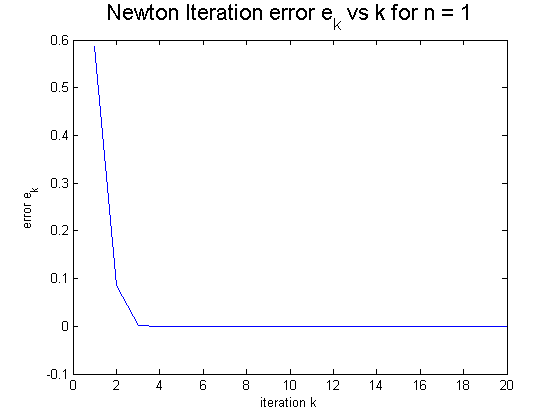
\includegraphics{n1} \\
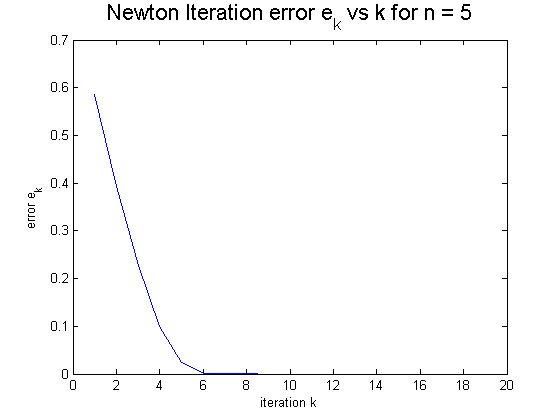
\includegraphics{n5} \\
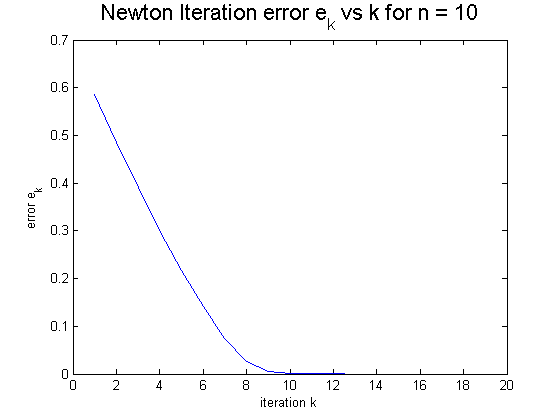
\includegraphics{n10} \\

You'll instantly notice that as $n$ grows, the convergence of the equation seems to slow. Since the convergence of this function is realized by Newton's Method, it has Quadratic Convergence. However, quadratically convergent equations have this truth: 
$$
\lim\limits_{k \rightarrow \infty} \frac{|e_{k+1}|}{|e_k|^2} = C
$$

Even though all Quadratically convergent equations have an increasing number correct digits per iteration, the constant $C$ determines how quickly the overall system converges (it modifies it by a constant factor, thereby ``stretching'' the error graph horizontally). And, if you'll recall from equation (15), this constant is given by $|\frac{g^{\prime\prime}(x^\star)}{2}|$. Therefore, it makes sense, since as $n$ grows, $|\frac{g^{\prime\prime}(x^\star)}{2}|$ grows.

\end{homeworkProblem}
\clearpage
%----------------------------------------------------------------------------------------
%	PROBLEM 7
%----------------------------------------------------------------------------------------

\begin{homeworkProblem}[Problem 7] % Roman numerals
	The code for this problem is included in the attached zip file as ``q7.m''.\\
	This instance of eigenvalue computation seems to work pretty well. I didn't find any instances where the algorithm diverged, even with a nearly-singular matrix. It often seemed to give the calculated eigenvectors in an opposite sign than did the QR method, at least for the matching eigenvector.
	
	An example,
	$$
	A = \left[\begin{array}{cc}
	1 & 3 \\
	1 & 7\\
	\end{array}\right]\\
	$$
	
	The algorithm returned $\lambda = 0.5359$, $\vec{v} = (0.9882, -0.1529)^T$ in one instance. However, since I initialized the starting vector randomly, sometimes it converged to the dominant eigenvalue/eigenvector pair.
\end{homeworkProblem}
\clearpage
\end{document}
